\appendix
\chapter{Tesztesetek}

\begin{figure}[H]
\begin{center}
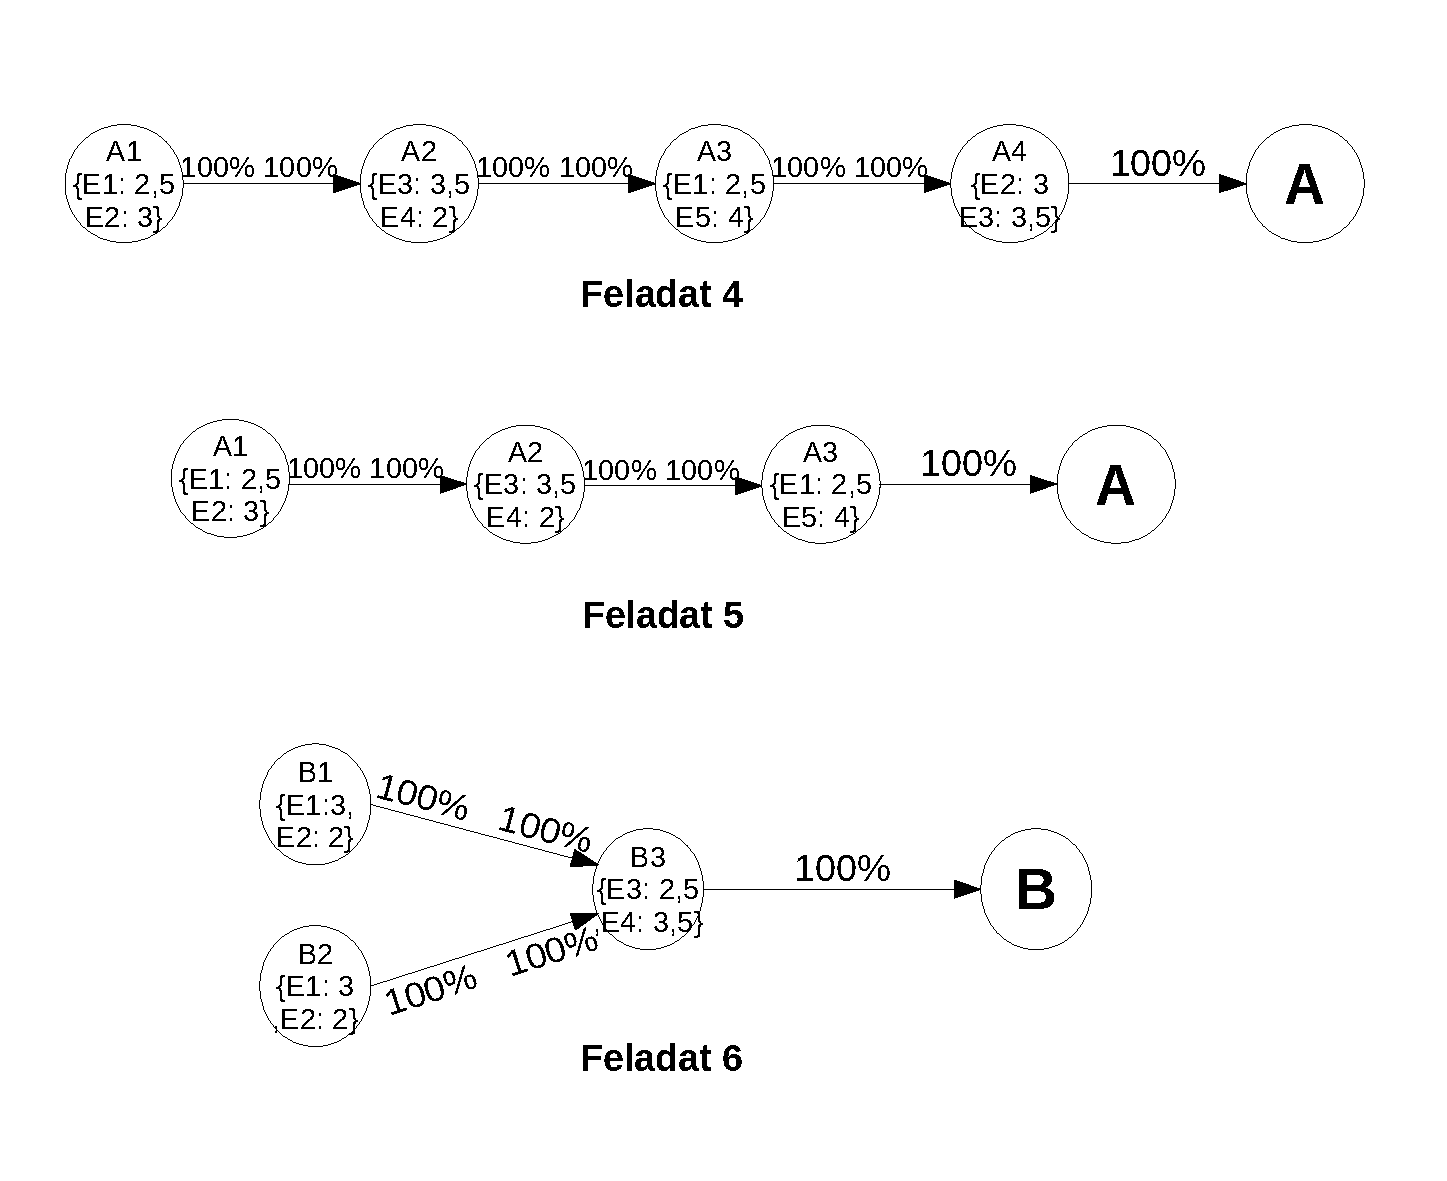
\includegraphics[scale=0.6]{tesztfeladatok2.pdf}
\caption{\ref{teszteredmenyek2} táblázatban szereplő feladatok}
\label{tesztfeladatok2}
\end{center}
\end{figure}

\begin{figure}[H]
\begin{center}
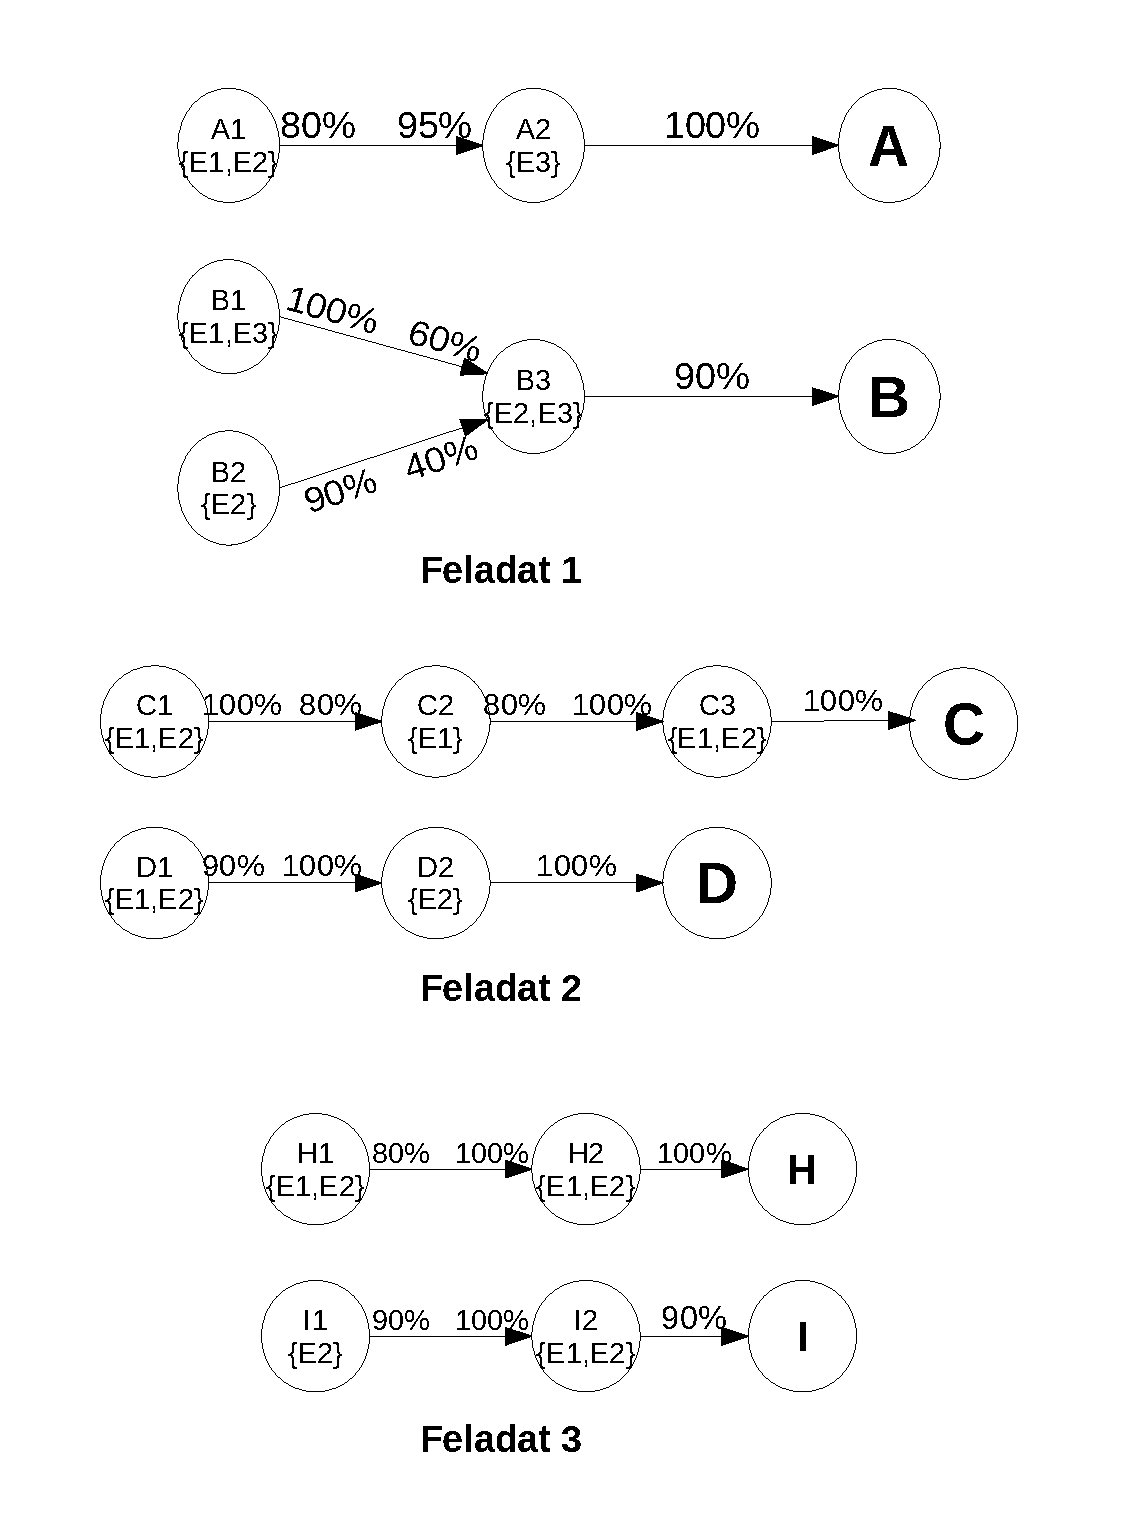
\includegraphics[scale=0.6]{tesztfeladatok.pdf}
\caption{\ref{teszteredmenyek} táblázatban szereplő feladatok}
\label{tesztfeladatok}
\end{center}
\end{figure}

\chapter{CD melléklet tartalma}
\dirtree{%
.1 CD\_melleklet.
.2 Felkeszules.
.3 MG\_Sgraf\_makespan.odg.
.3 MG\_Troughput\_maximization.odp.
.2 solver.
.3 input.
.4 extended\_precedential.ods.
.4 precedential.ods.
.3 src.
.4 lib.
.4 solver.
.2 Teszteles.
.3 Input\_fajlok.
.4 Feladat1.
.4 Feladat2.
.4 Feladat3.
.4 Feladat4.
.4 Feladat6.
.3 Megoldasok.
.4 Feladat1.
.4 Feladat2.
.4 Feladat3.
.4 Feladat4.
.4 Feladat6.
}




